\begin{figure}
\centering
\begin{subfigure}[t]{0.25\textwidth}
\centering
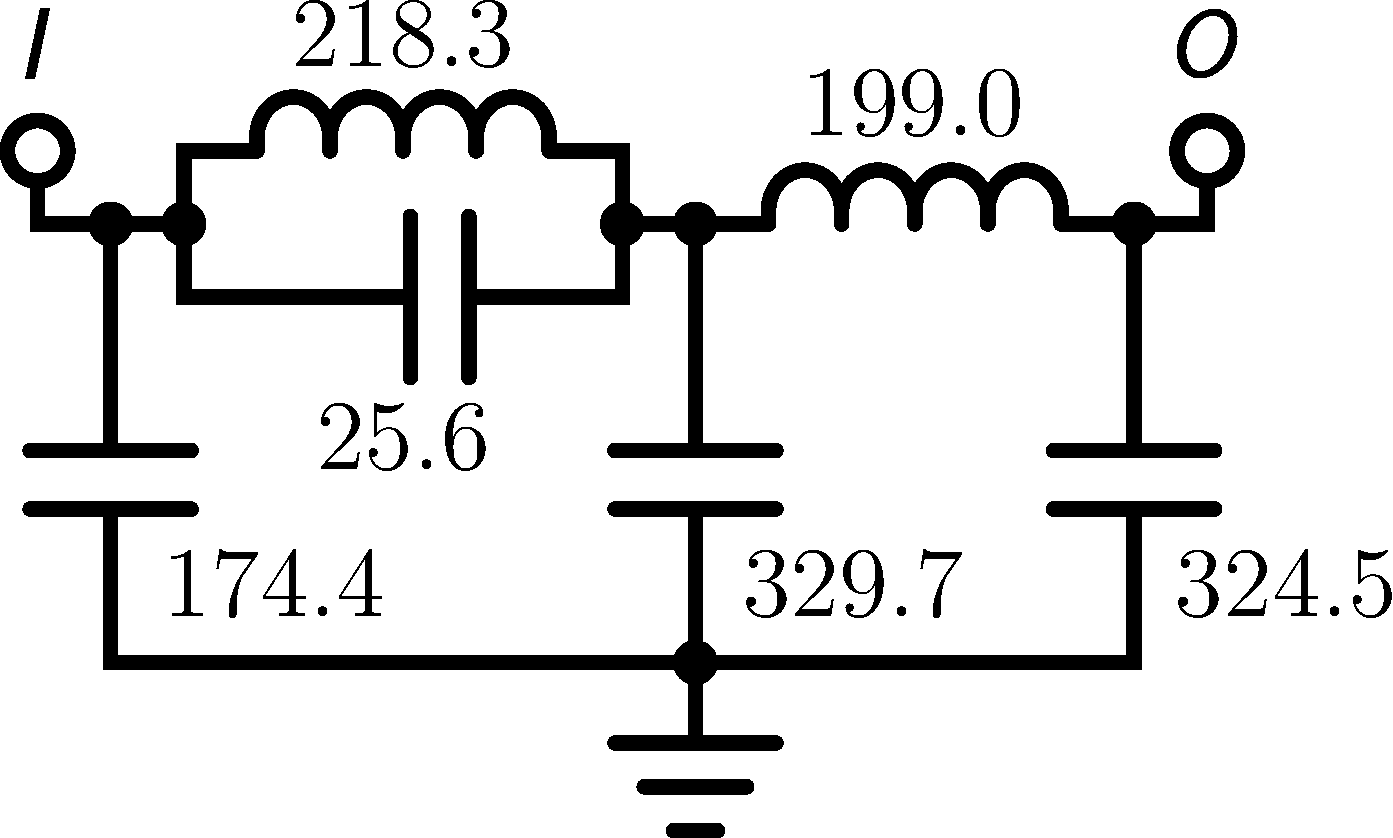
\includegraphics[scale = 0.14]{../ch6/figures/lpf2_circuit1}
\caption{\label{fig:lpf2_circuita}}
\end{subfigure}%
\begin{subfigure}[t]{0.25\textwidth}
\centering
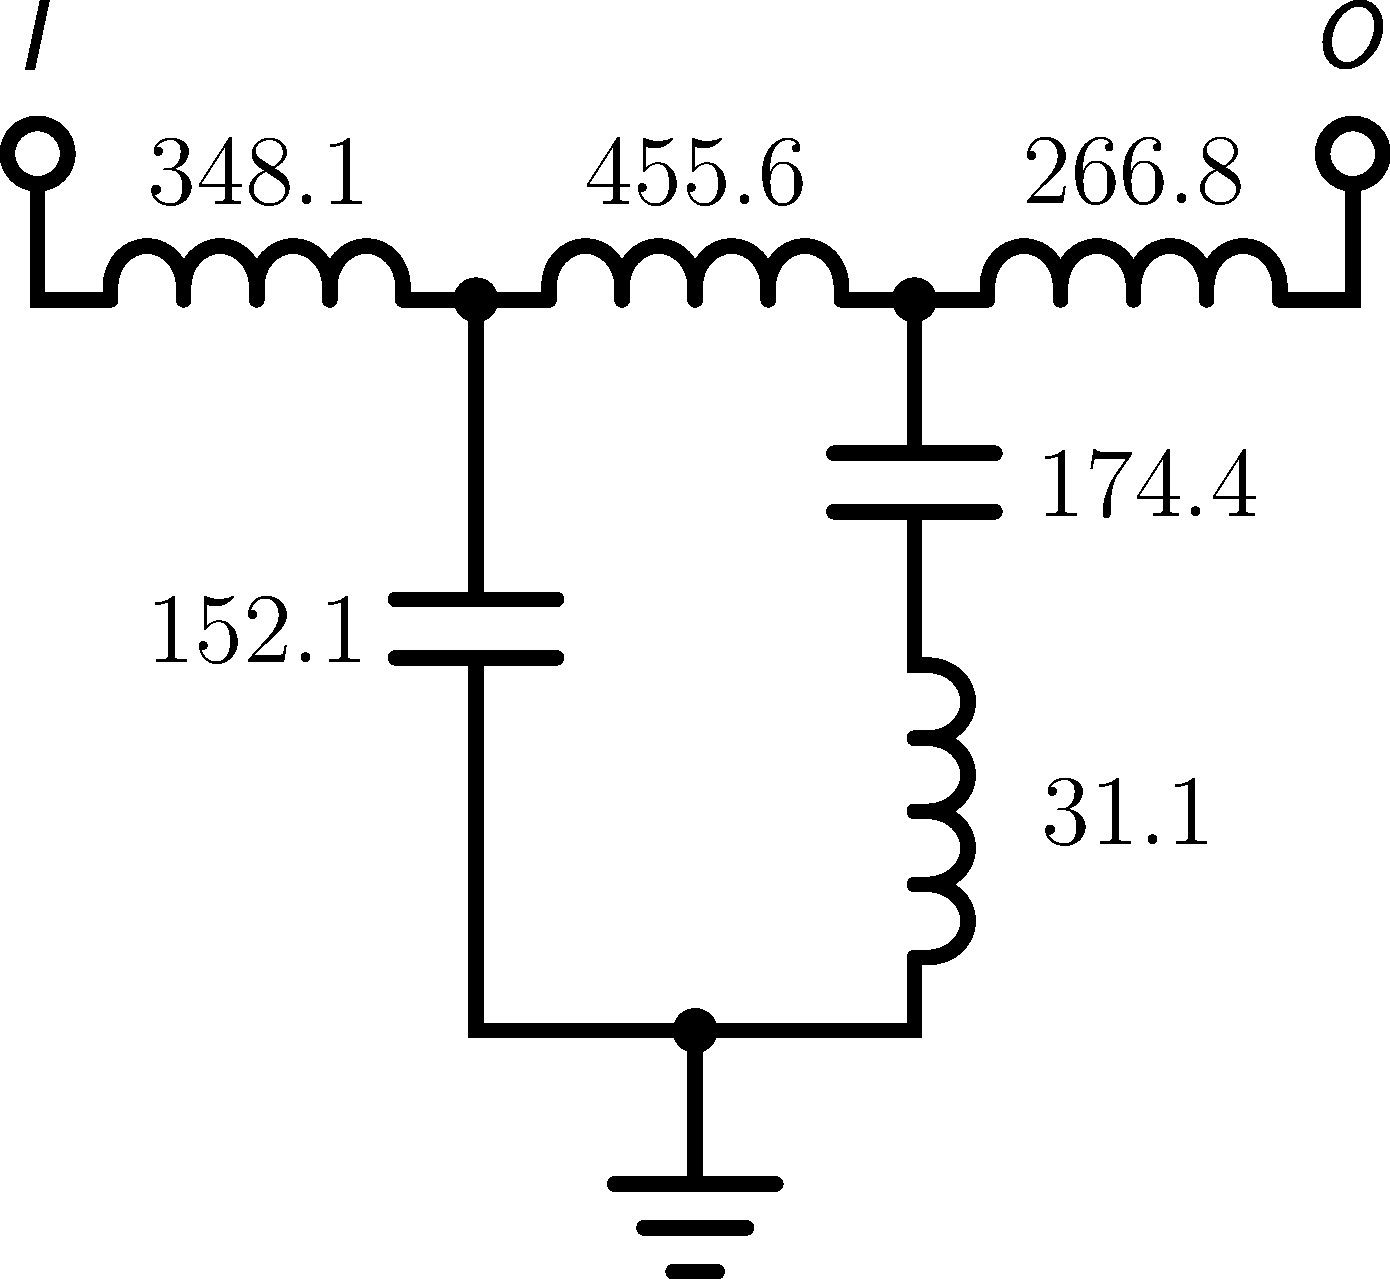
\includegraphics[scale = 0.14]{../ch6/figures/lpf2_circuit2}
\caption{\label{fig:lpf2_circuitb}}
\end{subfigure}%
% \vspace{0.06in}
\begin{subfigure}[t]{0.5\textwidth}
\centering
% 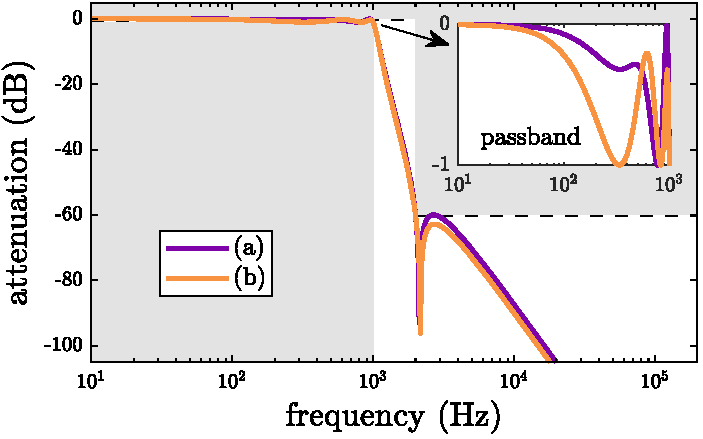
\includegraphics[width=\textwidth]{../ch6/figures/lpf2_magnitude}
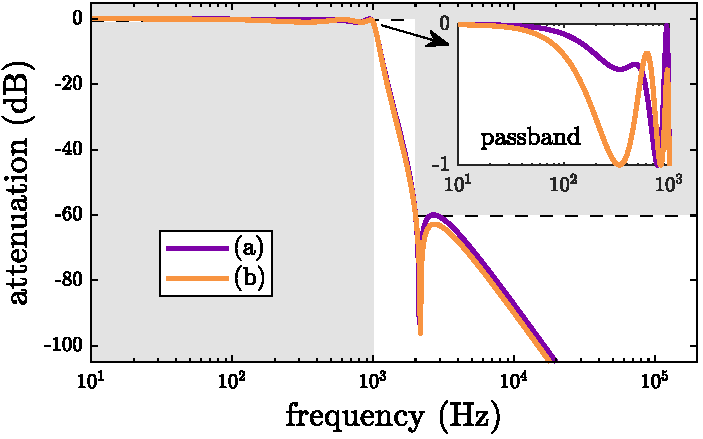
\includegraphics[width=\textwidth]{../ch6/figures/reduced/r_lpf2_magnitude}
\caption{\label{fig:lpf2_magnitude}}
\end{subfigure}%

\caption[Select feasible, minimum complexity circuits and attenuation responses for \nameref{sec:ch6:lpf} task \#2.]{Select feasible, minimum complexity circuits and attenuation responses for \nameref{sec:ch6:lpf} task \#2 (units are mH and nF).\label{fig:lpf2}}

\end{figure}